\documentclass{article}
\usepackage[margin=0.4in]{geometry}

\usepackage{tikz}
\usetikzlibrary{automata,positioning}
\begin{document}
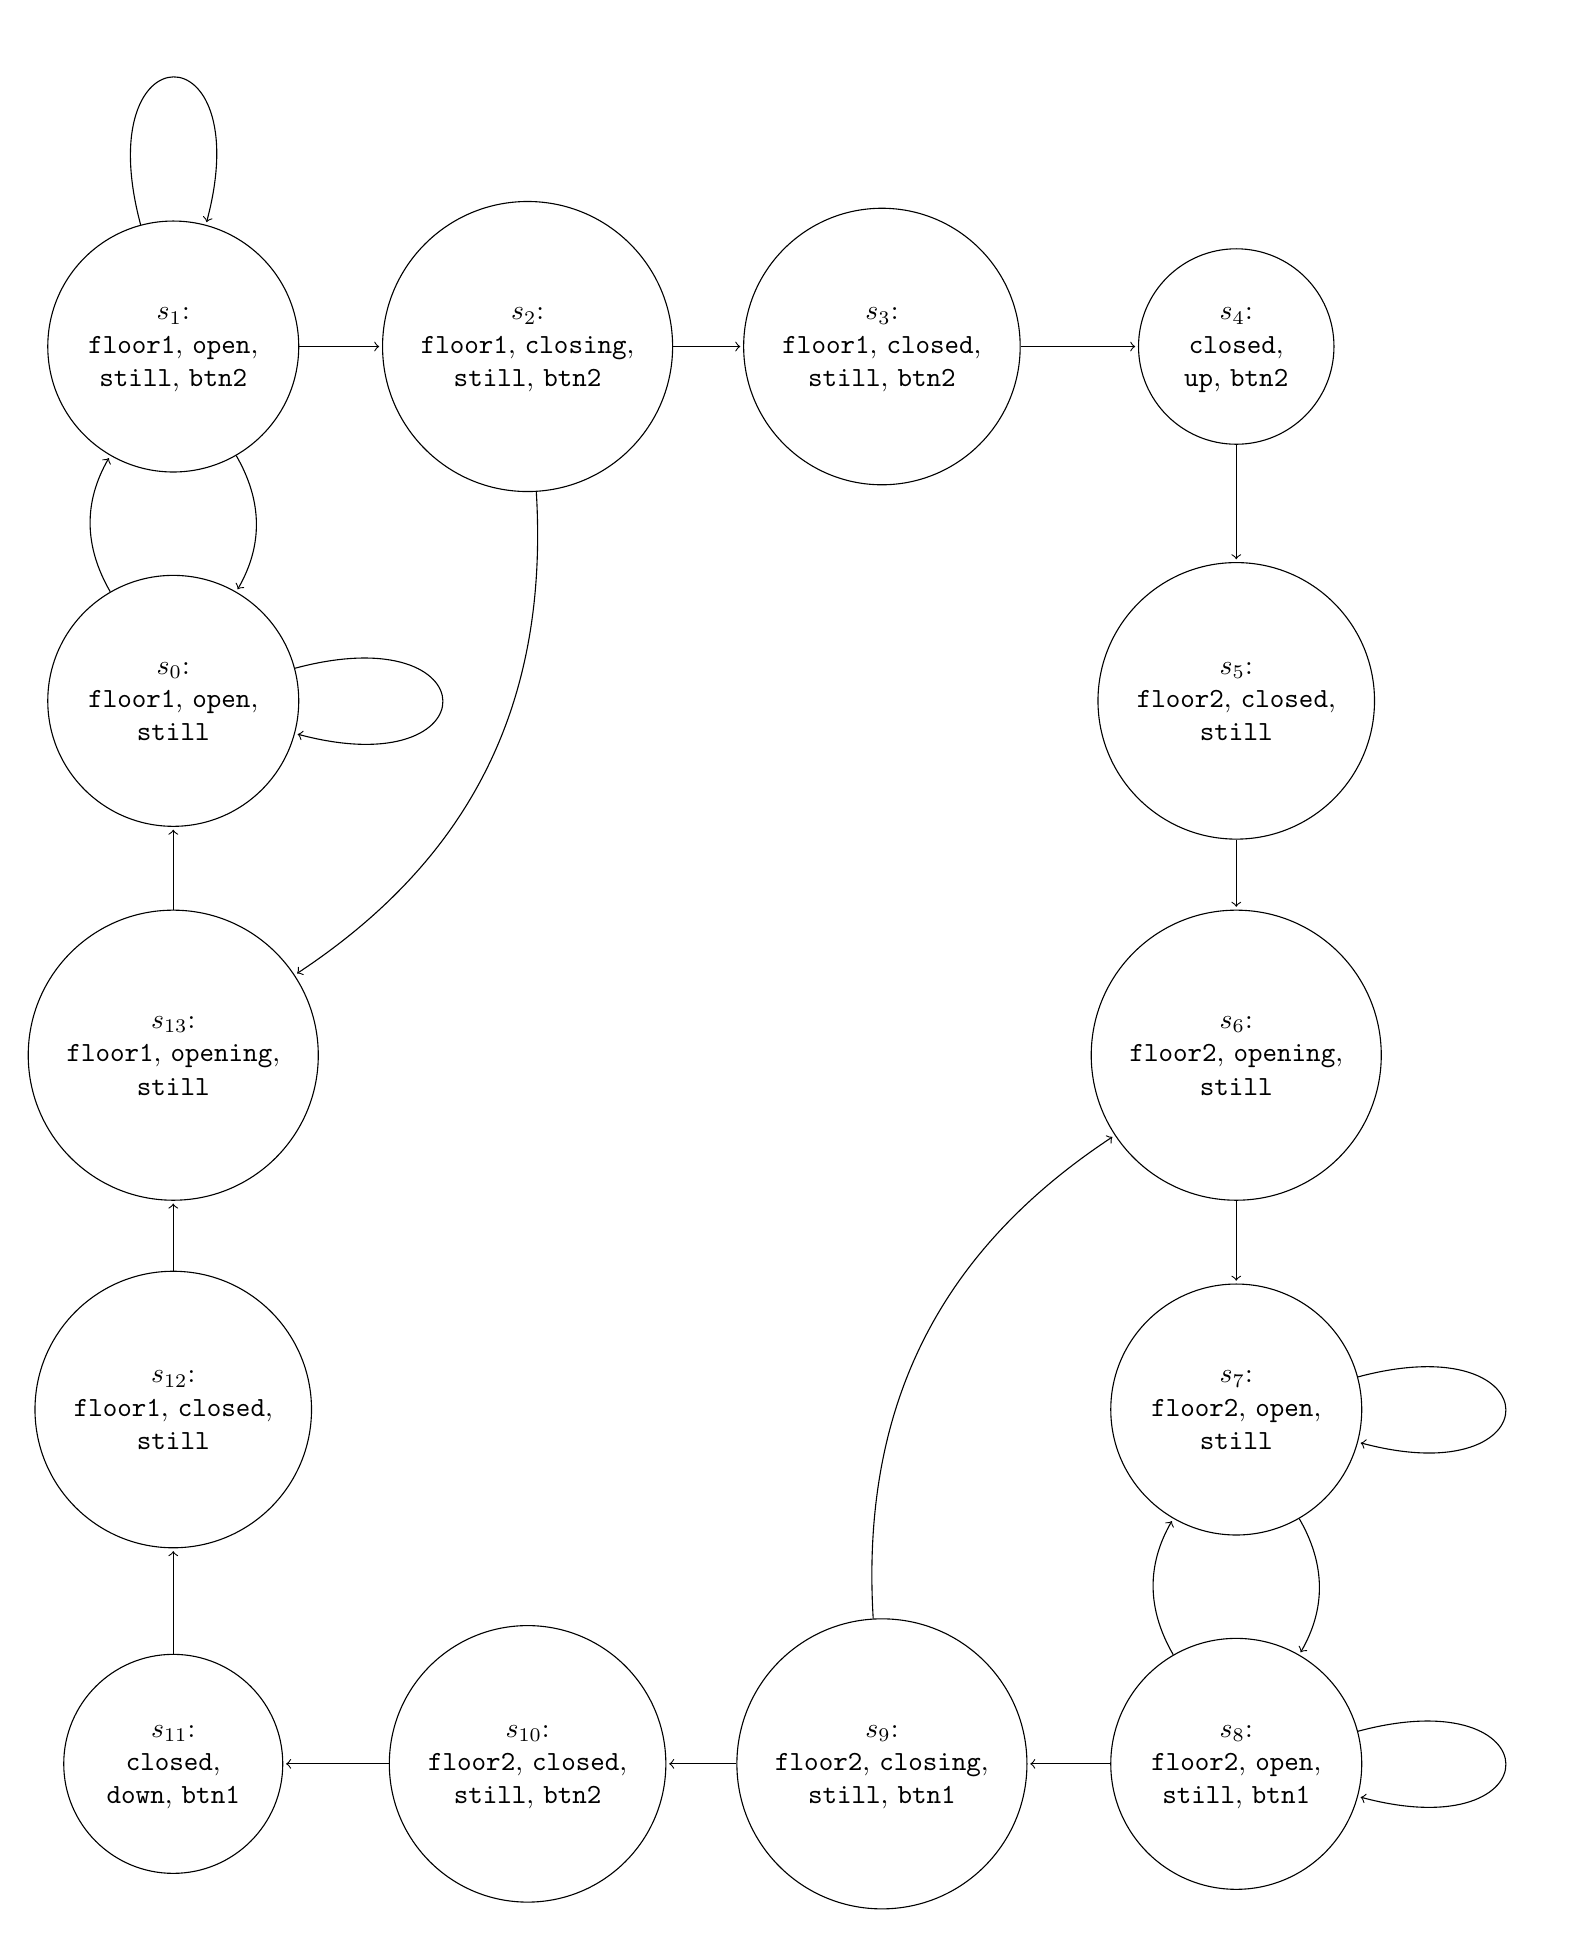
\begin{tikzpicture}[shorten >=1pt,node distance=2cm,on grid,auto] 
   \node[state] (s_0)   {\begin{tabular}{c}
    $s_0$: \\ 
      \texttt{floor1}, \texttt{open}, \\
      \texttt{still}
    \end{tabular}}; 
   \node[state] (s_1) [above=4.5cm of s_0] {\begin{tabular}{c}
    $s_1$: \\ 
      \texttt{floor1}, \texttt{open},\\
      \texttt{still}, \texttt{btn2}
    \end{tabular}};  
   \node[state] (s_2) [right=4.5cm of s_1] {\begin{tabular}{c}
    $s_2$: \\
      \texttt{floor1}, \texttt{closing},\\
      \texttt{still}, \texttt{btn2}
    \end{tabular}}; 
   \node[state] (s_3) [right=4.5cm of s_2] {\begin{tabular}{c}
   $s_3$: \\
      \texttt{floor1}, \texttt{closed},\\
      \texttt{still}, \texttt{btn2}
    \end{tabular}};
   \node[state] (s_4) [right=4.5cm of s_3] {\begin{tabular}{c}
    $s_4$: \\
      \texttt{closed}, \\
      \texttt{up}, \texttt{btn2}
    \end{tabular}};
   \node[state] (s_5) [below=4.5cm of s_4] {\begin{tabular}{c}
    $s_5$: \\
      \texttt{floor2}, \texttt{closed}, \\
      \texttt{still}
    \end{tabular}}; 
   \node[state] (s_6) [below=4.5cm of s_5] {\begin{tabular}{c}
    $s_6$: \\
      \texttt{floor2}, \texttt{opening}, \\
      \texttt{still}
    \end{tabular}}; 
   \node[state] (s_7) [below=4.5cm of s_6] {\begin{tabular}{c}
    $s_7$: \\
      \texttt{floor2}, \texttt{open}, \\
      \texttt{still}
    \end{tabular}}; 
   \node[state] (s_8) [below=4.5cm of s_7] {\begin{tabular}{c}
    $s_8$: \\
      \texttt{floor2}, \texttt{open}, \\
      \texttt{still}, \texttt{btn1}
    \end{tabular}}; 
   \node[state] (s_9) [left=4.5cm of s_8] {\begin{tabular}{c}
    $s_9$: \\
      \texttt{floor2}, \texttt{closing}, \\
      \texttt{still}, \texttt{btn1}
    \end{tabular}}; 
   \node[state] (s_10) [left=4.5cm of s_9] {\begin{tabular}{c}
    $s_{10}$: \\
      \texttt{floor2}, \texttt{closed}, \\
      \texttt{still}, \texttt{btn2}
    \end{tabular}}; 
   \node[state] (s_11) [left=4.5cm of s_10] {\begin{tabular}{c}
   $s_{11}$: \\
      \texttt{closed}, \\
      \texttt{down}, \texttt{btn1}
    \end{tabular}}; 
   \node[state] (s_12) [above=4.5cm of s_11] {\begin{tabular}{c}
   $s_{12}$: \\
      \texttt{floor1}, \texttt{closed}, \\
      \texttt{still}
    \end{tabular}}; 
   \node[state] (s_13) [below=4.5cm of s_0] {\begin{tabular}{c}
   $s_{13}$: \\
      \texttt{floor1}, \texttt{opening}, \\
      \texttt{still}
    \end{tabular}}; 
    \path[->] 
    (s_0) edge [bend left] node {} (s_1)
          edge [loop right] node {} ()
    (s_1) edge [bend left] node  {} (s_0) 
          edge [loop above] node {} ()
          edge node {} (s_2)
    (s_2) edge node [swap] {} (s_3) 
          edge [bend left] node {} (s_13)
    (s_3) edge node [swap] {} (s_4)
    (s_4) edge node [swap] {} (s_5)
    (s_5) edge node [swap] {} (s_6)
    (s_6) edge node [swap] {} (s_7) 
    (s_7) edge [bend left] node [swap] {} (s_8)
          edge [loop right] node {} ()
    (s_8) edge [bend left] node [swap] {} (s_7)
          edge [loop right] node {} ()
          edge node [swap] {} (s_9)
    (s_9) edge [bend left] node [swap] {} (s_6)
          edge node [swap] {} (s_10)
    (s_10) edge node [swap] {} (s_11)
    (s_11) edge node [swap] {} (s_12) 
    (s_12) edge node [swap] {} (s_13)
    (s_13) edge node [swap] {} (s_0); 
\end{tikzpicture}
\end{document}
